\documentclass{article}
\usepackage[polish]{babel}
\usepackage{titling}
\usepackage[T1]{fontenc}

% Margins in document
\usepackage[left=1.5cm, right=1.5cm, top=3cm]{geometry}

% Avoid  colons before tables' empty captions and change caption
\usepackage{caption}
\captionsetup[table]{name=Tab.}
\captionsetup[figure]{name=Rys.}

% Don't know why, it starts from 2
\addtocounter{table}{-1}

% Rename tables' suffix
\renewcommand{\tablename}{Tab.}

% Graphicx setup
\usepackage{graphicx}
\graphicspath{{grafiki/}{../grafiki/}}

% No separator between items
\usepackage{enumitem}
\setlist{nolistsep}

% Pagebreak before every \section
\let\oldsection\section
\renewcommand\section{\clearpage\oldsection}

% Vhistory setup
\usepackage[owncaptions]{vhistory}
\renewcommand{\vhhistoryname}{Historia zmian}
\renewcommand{\vhversionname}{Wersja}
\renewcommand{\vhdatename}{Data}
\renewcommand{\vhauthorname}{Autor(zy)}
\renewcommand{\vhchangename}{Zmiany}

% Bigger padding in tabulars
\usepackage{array}
\setlength\extrarowheight{3pt}

% Itemize in tabulars (avoid big margins with minipage)
\newcommand{\tabbeditemize}[1]{
	\begin{minipage}[t]{0.4\textwidth}
		\begin{itemize}[topsep=0mm,partopsep=0mm,leftmargin=4mm]
			#1
		\end{itemize}
\end{minipage}}


% DOCUMENT
\title{
	Wizualizacja drzewa stanów algorytmu UCT \\
	\large Dokumentacja wymagań projektu}

\author{Patryk Fijałkowski \\ Grzegorz Kacprowicz}
\begin{document}
	\begin{titlingpage}
		\maketitle
		\vspace{3cm}
		\begin{abstract}
			Dokument opisuje ogólne założenia stworzenia projektu wizualizacji drzew stanów algorytmu z dziedziny sztucznej inteligencji - Upper Confidence Bound Applied to Trees. Krytyczne dla skuteczności tytułowej heurystyki są odpowiednia konstrukcja i trawersowanie generowanych drzew. Nasze rozwiązanie wykorzysta ten algorytm w podejmowaniu decyzji podczas grania w dwie przykładowe gry planszowe. Skupimy się na przejrzystej wizualizacji, ukazując kolejne etapy rozrastania się drzew. Finalna wersja aplikacji będzie wygodnym narzędziem do analizy działania algorytmu w czasie rzeczywistym. Przeprowadzana w dokumencie analiza wykazała, że mogą wystąpić typowe ryzyka, które nie wpłyną znacząco na terminy realizacji projektu.
		\end{abstract}
	\end{titlingpage}

	\begin{versionhistory}
		\vhEntry{1.0}{19.10.2019}{PF|GK}{stworzenie pierwszej wersji dokumentu}
		\vhEntry{1.1}{23.10.2019}{PF|GK}{korekty po uwagach promotora pracy}
		\vhEntry{1.2}{23.10.2019}{PF|GK}{korekty po uwagach promotora pracy}
		\vhEntry{1.3}{23.10.2019}{PF}{drobne korekty po uwagach promotora pracy}
	\end{versionhistory}
	
	\tableofcontents
	
		
	\section{Słownictwo}
	\begin{itemize}
		\item \textbf{MCTS} (Monte Carlo Tree Search) - heurystyka podejmowania decyzji w pewnych zadaniach sztucznej inteligencji, np. ruchów w grach. Najczęściej MCTS opiera się na jakimś wariancie metody UCT.
		\item \textbf{UCT} (Upper Confidence Bound Applied to Trees) - algorytm przeszukujący drzewo stanów rozgrywki w poszukiwaniu najbardziej opłacalnych ruchów. Algorytm stara się zachować równowagę między eksploatacją ruchów po ruchach o wysokiej średniej wygranej a eksploracją tych mało sprawdzonych.
		\item \textbf{Podstawowa wizualizacja} - możliwość wyświetlenia wszystkich wierzchołków drzewa. W podstawowej wizualizacji wygląd wierzchołków jest nieistotny.
		\item \textbf{Zaawansowana wizualizacja} - podstawowa wizualizacja wzbogacona o możliwość analizowania statystyk poszczególnych wierzchołków. Kolor wierzchołków będzie reprezentował aktualnego gracza.
		\item \textbf{Pełna wizualizacja} - zaawansowana wizualizacja wzbogacona o możliwość przewijania, przybliżania oraz oddalania podglądu drzewa.
	\end{itemize}


	\oldsection{Cel biznesowy}
	Algorytm UCT, będący usprawnieniem MCTS, jest powszechnie stosowanym algorytmem w sztucznej inteligencji. Jest metodą analizującą obiecujące ruchy na podstawie generowanego drzewa, która równoważy eksploatację najbardziej korzystnych z eksploracją mniej korzystnych decyzji. Każdemu wierzchołkowi drzewa odpowiada pewien stan rozgrywki, z którego algorytm rozgrywa losowe symulacje, rozszerzając potem drzewo o kolejne możliwe stany. Sposób, w jaki rozrasta się opisywane drzewo, jest kluczowy dla podejmowania przez algorytm jak najlepszych decyzji.\\\\
	\noindent Celem projektu jest stworzenie aplikacji pozwalającej na wizualizację drzew algorytmu UCT. Aplikacja będzie pozwalała na wizualizowanie drzew generowanych podczas rozgrywania dwóch przykładowych gier (pozwalając przetestować rozwiązanie). Aplikacja powinna pozwalać na wizualizację drzew, ich sekwencji i róznic między kolejnymi drzewami w sekwencji. Powinna być możliwość płynnego przybliżania/oddalania i przewijania wizualizacji oraz zapisu aktualnego stanu do pliku graficznego - wszystko, aby klient mógł wygodnie korzystać z naszego programu.\\\\
	Taki produkt pozwoliłby zrozumieć klientowi ideę i sposób działania algorytmu UCT.
	

	
	
	\section{Wymagania funkcjonalne}
	Użytkownik korzystający z naszej aplikacji będzie mógł wybrać jedną z dwóch gier deterministycznych, a do wyboru będzie miał dwa tryby rozgrywki:
	\begin{enumerate}
		\item Gracz vs PC - gdzie użytkownik będzie decydował o swoich posunięciach i zmierzy się on z zaimplementowanym algorytmem,
		\item PC vs PC - gdzie będzie on de facto świadkiem symulacji algorytmu, który rozgrywa partię z samym sobą.\\
	\end{enumerate}
	Zanim jednak przejdzie do rozgrywki, będzie miał możliwość ustawienia parametrów algorytmu, tj. liczbę iteracji podczas tworzenia drzewa czy też maksymalny czas na ruch przeciwnika (co też wiąże się z liczbą iteracji).
	Druga opcja, którą będzie dysponować użytkownik, to możliwość wczytania drzewa w formacie zarówno binarnym jak i CSV.
	a następnie możliwość jego dogłębnej analizy. Będzie on mógł wyświetlać informacje na temat wybranego węzła, a także przybliżać i oddalać cały wygenerowany graf. Podczas samej rozgrywki gracz będzie mógł wyeksportować drzewo po wykonanym ruchu przeciwnika i analizować je w sposób opisany powyżej. Tak samo, będzie też miał możliwość zapisania go w wyżej wymienionych formatach, a także w formacie rastrowym. Użytkownik będzie mógł oglądać rozrost drzewa.
	Dodatkowo, będzie mógł porównać nowo wygenerowane drzewo z tym z poprzedniego kroku.  Powyższe rzeczy dotyczą obu trybów gry i każdej z gier. \\\\
	Diagram przypadków użycia, który ilustruje przedstawione możliwości, znajduje się na rysunku \ref{rys:usecase}.

	\begin{figure}[h!]
		\centering
		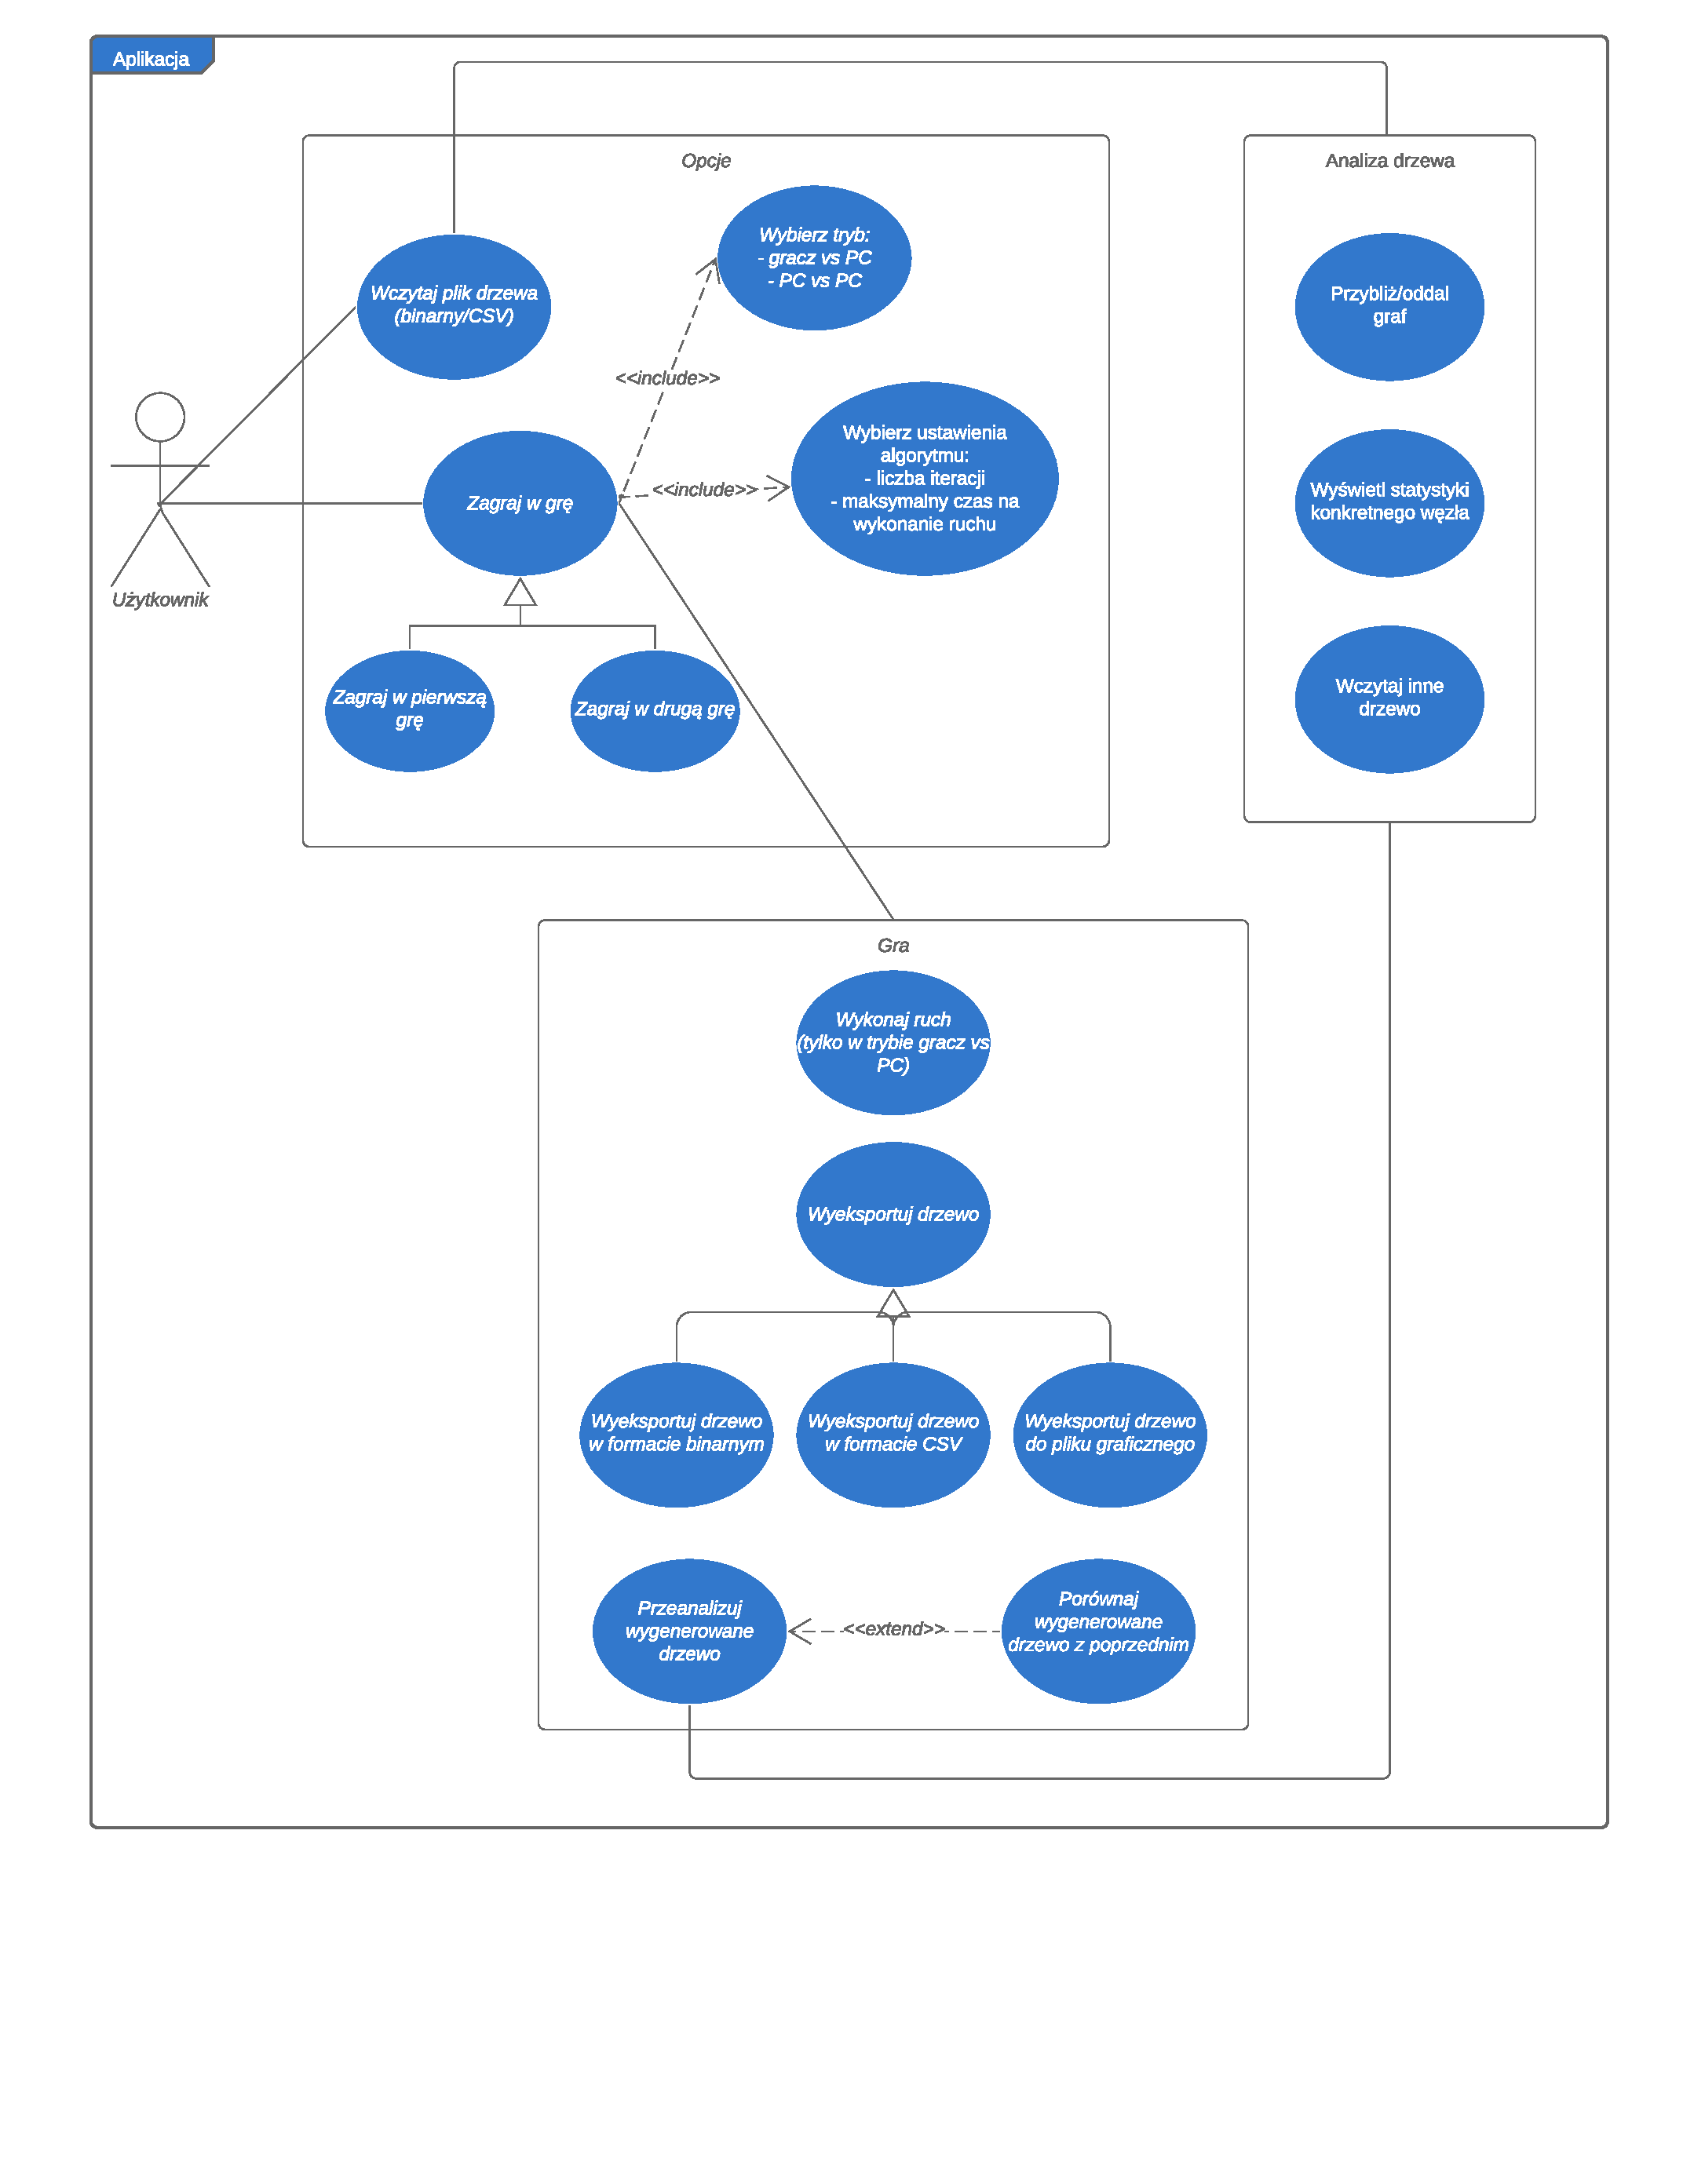
\includegraphics[width=\textwidth, trim={0 6.5cm 0 0},clip]{aplikacja-use-case-eps}
		\caption{Diagram przypadków użycia}
		\label{rys:usecase}
	\end{figure}
	
	\section{Wymagania niefunkcjonalne}
	Wymagania niefunkcjonalne opisane są w tabeli \ref{tab:furps} przy użyciu metody FURPS. Zawiera ona między innymi opis wymagań sprzętowych aplikacji oraz jej ograniczenia wydajnościowe. Celem analizy wymagań jest jednoznaczne określenie zakresu prac i ułatwienie nam podejmowania decyzji w zakresie wybieranych rozwiązań architektonicznych.

	\begin{table}[h!]
	\centering
	\begin{tabular}{|l|p{0.7\linewidth}|}
		\hline
		Obszar         & \textbf{Opis} \\ \hline
		Funkcjonalność & Aplikacja będzie potrzebować komputera z odpowiednim środowiskiem uruchomieniowym dla aplikacji oraz procesor graficzny. Ponadto, wymagana jest zainstalowana biblioteka OpenGL w wersji 2.0. Dostęp do sieci nie jest potrzebny dla poprawnego działania aplikacji.  \\ \hline
		Używalność     & Aplikacja będzie działać w kilku oknach wyposażonych w przejrzysty interfejs dla użytkownika. Ponadto, zostanie dostarczona obszerna dokumentacja aplikacji, w której zostanie zawarta instrukcja obsługi.  \\ \hline
		Niezawodność   & Aplikacja będzie działać na komputerze lokalnym, więc będzie dostępna cały czas. Wszelkie błędy powinny być obsłużone wewnątrz aplikacji.  \\ \hline
		Wydajność      & Aplikacja będzie korzystała głównie z pamięci RAM, procesora i procesora graficznego. Maksymalna dopuszczalna liczba wierzchołków analizowanych drzew to $500 \,\,000$. W przypadku dużych drzew (o liczbie wierzchołków bliskiej maksymalnej) powinna odpowiadać z opóźnieniem maksymalnie 1s, a dla drzew do $100\,\,000$ wierzchołków - z opóźnieniem do 200ms.  \\ \hline
		Wsparcie       & Aplikacja będzie przeznaczona dla komputerów z systemami operacyjnymi Windows, Linux oraz MacOS. Aplikacja nie będzie rozszerzalna - wszystkie obliczenia i wizualizacje będą przeprowadzone wewnątrz jednej maszyny.  \\ \hline
	\end{tabular}
	\caption{Analiza FURPS}
	\label{tab:furps}
	\end{table}
	
	
	\section{Harmonogram}
	\subsection{Tabela}
	Pracę nad projektem opisuje harmonogram z tabeli \ref{tab:schedule}. Tabela nie opisuje zależności między kolejnymi fazami rozwoju projektu, wyznacza jedynie planowe terminy ich zakończenia. Tworząc tabelę, staraliśmy się rozłożyć pracę regularnie na cały zaplanowany czas tworzenia projektu. Zostawiliśmy również ostatnie 2 tygodnie na doszlifowanie elementów, z którymi potencjalnie nie wyrobilibyśmy się na czas.
	\begin{table}[h!]
	\centering
	\begin{tabular}{|l|l|}
		\hline
		\textbf{Deadline}   & \textbf{Przygotowane zadania}                                                         \\ \hline
		24.10.2019 & \tabbeditemize{\item Serializacja \item Algorytm \item Pierwsza gra} \\ \hline
		7.11.2019  & \tabbeditemize{\item Podstawowa wizualizacja \item Połączenie algorytmu i gry}\\ \hline
		21.11.2019 & \tabbeditemize{\item Zaawansowana wizualizacja \item Aplikacja okienkowa \item Zapis drzew do pliku graficznego} \\ \hline
		5.12.2019  & \tabbeditemize{\item Pełna wizualizacja \item Druga gra} \\ \hline
		19.12.2019 & \tabbeditemize{\item Usprawnienia, poprawki}\\ \hline
	\end{tabular}
	\caption{Harmonogram pracy}
	\label{tab:schedule}
	\end{table}

	\subsection{Diagram Gantta}
	\noindent Aby dobrze zwizualizować zależności pomiędzy kolejnymi etapami rozwoju aplikacji, sporządziliśmy diagram Gantta, przedstawiony na rysunku \ref{rys:gantt}.
	
	\begin{figure}[h]
		\centering
		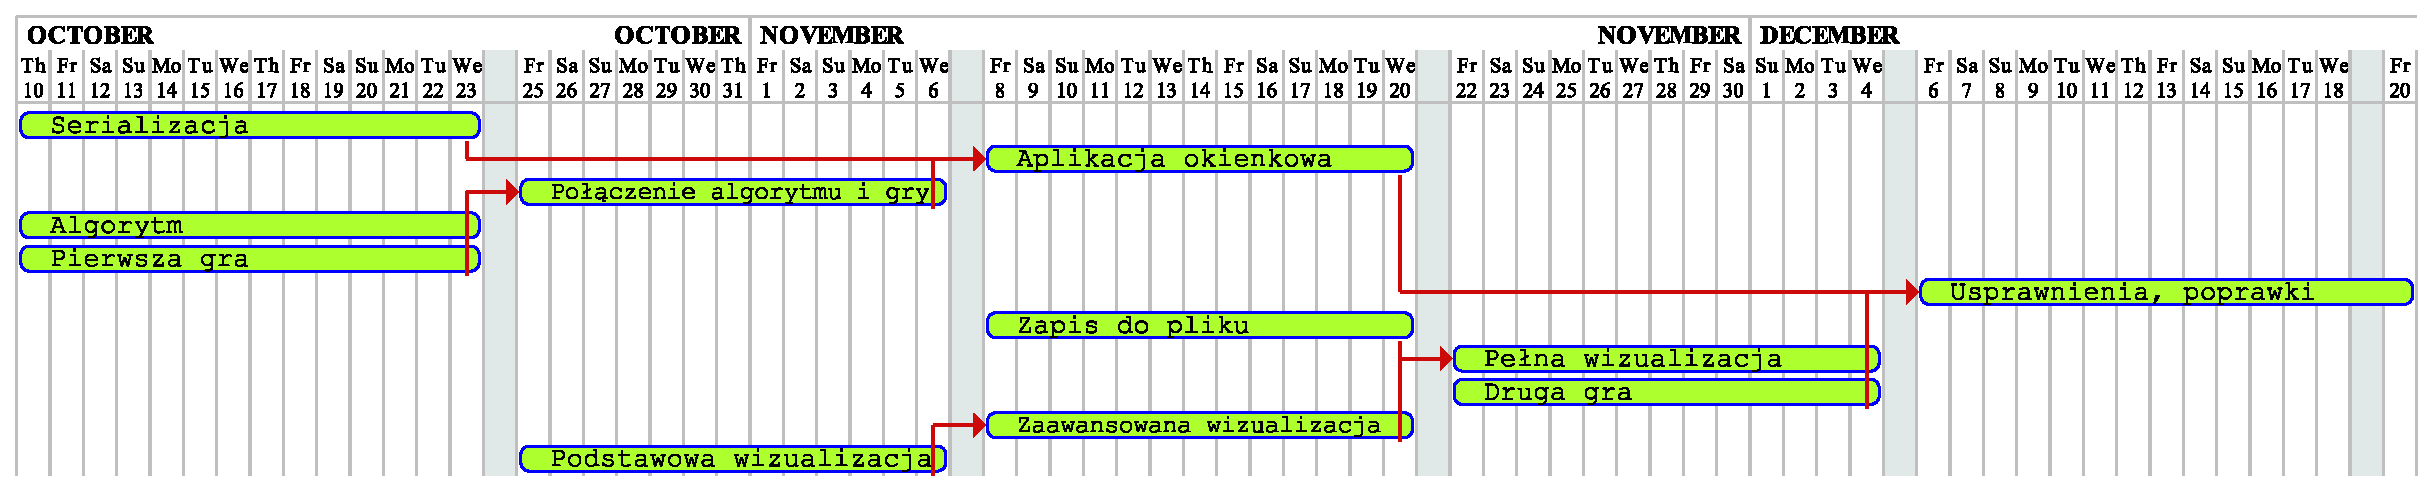
\includegraphics[width=\textwidth]{gantt}
		\caption{Diagram Gantta}
		\label{rys:gantt}
	\end{figure}

	\noindent Jak widać na diagramie, jedynymi z najbardziej kluczowych punktów podczas rozwoju projektu są \texttt{połączenie algorytmu i gry} oraz elementy związane z \texttt{wizualizacją}. Elementy takie jak \texttt{druga gra} czy \texttt{zapis do pliku} są najmniej istotnymi punktami z punktu widzenia powodzenia projektu. Ostatnie 2 planowane tygodnie planujemy poświęcić na \texttt{usprawnienia i poprawki}, zostawiając sobie w ten sposób czas na dopracowanie komponentów, które zostały zaplanowane wcześniej i nie zostały stworzone wystarczająco dobrze.
		
	
	\section{Analiza ryzyka}
	
	\begin{table}[h!]
	\centering
	\bgroup
	\def\arraystretch{1.5}% 
	\begin{tabular}{|l|l|l|}
		\hline
		& \textbf{Czynniki pozytywne} & \textbf{Czynniki negatywne} \\
		\hline
		\textbf{Czynniki wewnętrzne}	& 

		\begin{minipage} [t] {0.35\textwidth} 
			Atuty:
		\begin{itemize}
			\item gotowość do ciężkiej pracy
			\item motywacja
			\item sumienność
			\item dobrze przygotowany plan
			\item wzajemne wsparcie i pomoc\\
		\end{itemize} 
		
		\end{minipage} & \begin{minipage} [t] {0.35\textwidth} 
		Słabości:
		\begin{itemize}
			\item ograniczona ilość czasu, który możemy poświęcić na projekt
			\item życie studenckie
			\item życie prywatne\\
		\end{itemize} 
		
	\end{minipage} \\
		\hline
		\textbf{Czynniki zewnętrzne}	&  \begin{minipage} [t] {0.35\textwidth} 
			Szanse:
			\begin{itemize}
				\item współpraca z promotorem
			\end{itemize} 
			
		\end{minipage} & \begin{minipage} [t] {0.35\textwidth} 
		Zagrożenia:
		\begin{itemize}
			\item ograniczenia płynące z wybranych technologii
			\item wybrane technologie mogą nie działać w oczekiwany sposób
			\item potencjalna trudność w połączeniu stworzonych komponentów aplikacji\\
		\end{itemize} 
		
	\end{minipage} \\
		\hline
	\end{tabular}
	\egroup
	\caption{Analiza SWOT}
	\label{tab:swot}
	\end{table}

	\noindent Tabela \ref{tab:swot} z analizą SWOT z grubsza określa różne czynniki, które będą miały kluczowy wpływ na przebieg naszego procesu tworzenia aplikacji. O ile jest dużo pozytywnych czynników, które na pewno pomogą nam w tym procesie, to tych negatywnych również nie brakuje i ważną dla nas sprawą jest znalezienie sposobu, aby się ich skutecznie wystrzec.\\\\
	Wybraną przez nas technologią do napisania aplikacji (gier, algorytmu, wizualizacji) jest język programowania \textbf{Python}. Do implementacji gier będziemy posługiwać się biblioteką \textbf{PyGame} w stabilnej wersji, która jest do tego celu przeznaczona i jest popularna. Wizualizacja będzie wykorzystywać w znacznym stopniu bibliotekę \textbf{VisPy} (OpenGL), gdzie można tworzyć również kod w języku \textbf{C++} - najprawdopodobniej będzie to najbardziej problematyczna technologia.
	Python będzie używany w najnowszej stabilnej wersji - 3.7 - jest to zaufana technologia.\\
	
	\noindent VisPy jest nową technologią, która jest wciąż rozwijana. Wybraliśmy ją ze względu na to, że
	\begin{itemize}
		\item współpracuje z GPU, co znakomicie przyspiesza rysowanie wizualizacji,
		\item posiada obszerną dokumentację,
		\item nie znaleźliśmy lepszej alternatywy (inne były najczęściej niezadowalające).\\
	\end{itemize}
	Ryzyko:
	\begin{enumerate}
		\item Nie znamy składni biblioteki OpenGL i jej nauka może zająć stosunkowo dużo czasu. Solucja: zaplanujemy i poświęcimy odpowiednią ilość czasu na testowanie i naukę potrzebnych nam funkcji.
		\item VisPy może okazać się wadliwe. W takiej sytuacji szukalibyśmy sprytnych obejść, a w najgorszym wypadku znajdziemy inną bibliotekę.
		\item Trudność w połączeniu komponentów - być może nie będą one działać w jednym oknie, połączenie może być bardzo czasochłonne lub sposób wymiany danych między komponentami będzie nieefektywny. Solucja: odpowiednio rozplanowany czas, który pozwoli na dobre zaplanowanie i wdrożenie optymalnej architektury. 
	\end{enumerate}
\end{document}